\chapter{Implementation and Integration in Robots}
\label{chapter|implementation_integration}

\section{Some implementation notes}

This section presents some of the main technological choices that have
been made to implement the knowledge base.

Some of the main algorithms are presented here as well (like the algorithms for clasification and discrimination,~\ref{sect|discrinimation}).

\subsection{A centralized server-based implementation}
\label{sect|oro-serverbased}


\subsection{OWL-DL ontologies and Jena}
\label{sect|jena}

\subsection{Reasoning: the Pellet reasoner}
\label{sect|pellet}

\subsection{Classification and discrimination algorithms}
\label{sect|discrimination}

%%%%%%%%%%%%%%%%%
\section{Bindings to other components/languages}
\label{sect|interfacing}

%%%%%%%%%%%%%%%%%
\section{Monitoring and debugging}
\label{sect|monitoring}

\subsection{Logging}

\subsection{Vizualisation}

oro-view, DOT export...

%%%%%%%%%%%%%%%%%
\section{Integration in the robot architecture}

\subsection{RPC and events-oriented interactions}

\subsection{Acquiring and Anchoring Knowledge in the physical world: the SPARK module}

\subsubsection{Building an Agent-Aware Symbolic Model of the Environment}
\label{sect|situ}

Anchoring perceptions in a symbolic model requires perception abilities and
their symbolic interpretation. In this section we present SPARK (\emph{SPAtial
Reasoning \& Knowledge}~\cite{Sisbot2011}), a situation assessment reasoner
that generates relevant symbolic information from the geometry of the
environment with respect to relations between objects, robots and humans.

\begin{figure}[ht!]
   \begin{center}
%
       \subfigure{
           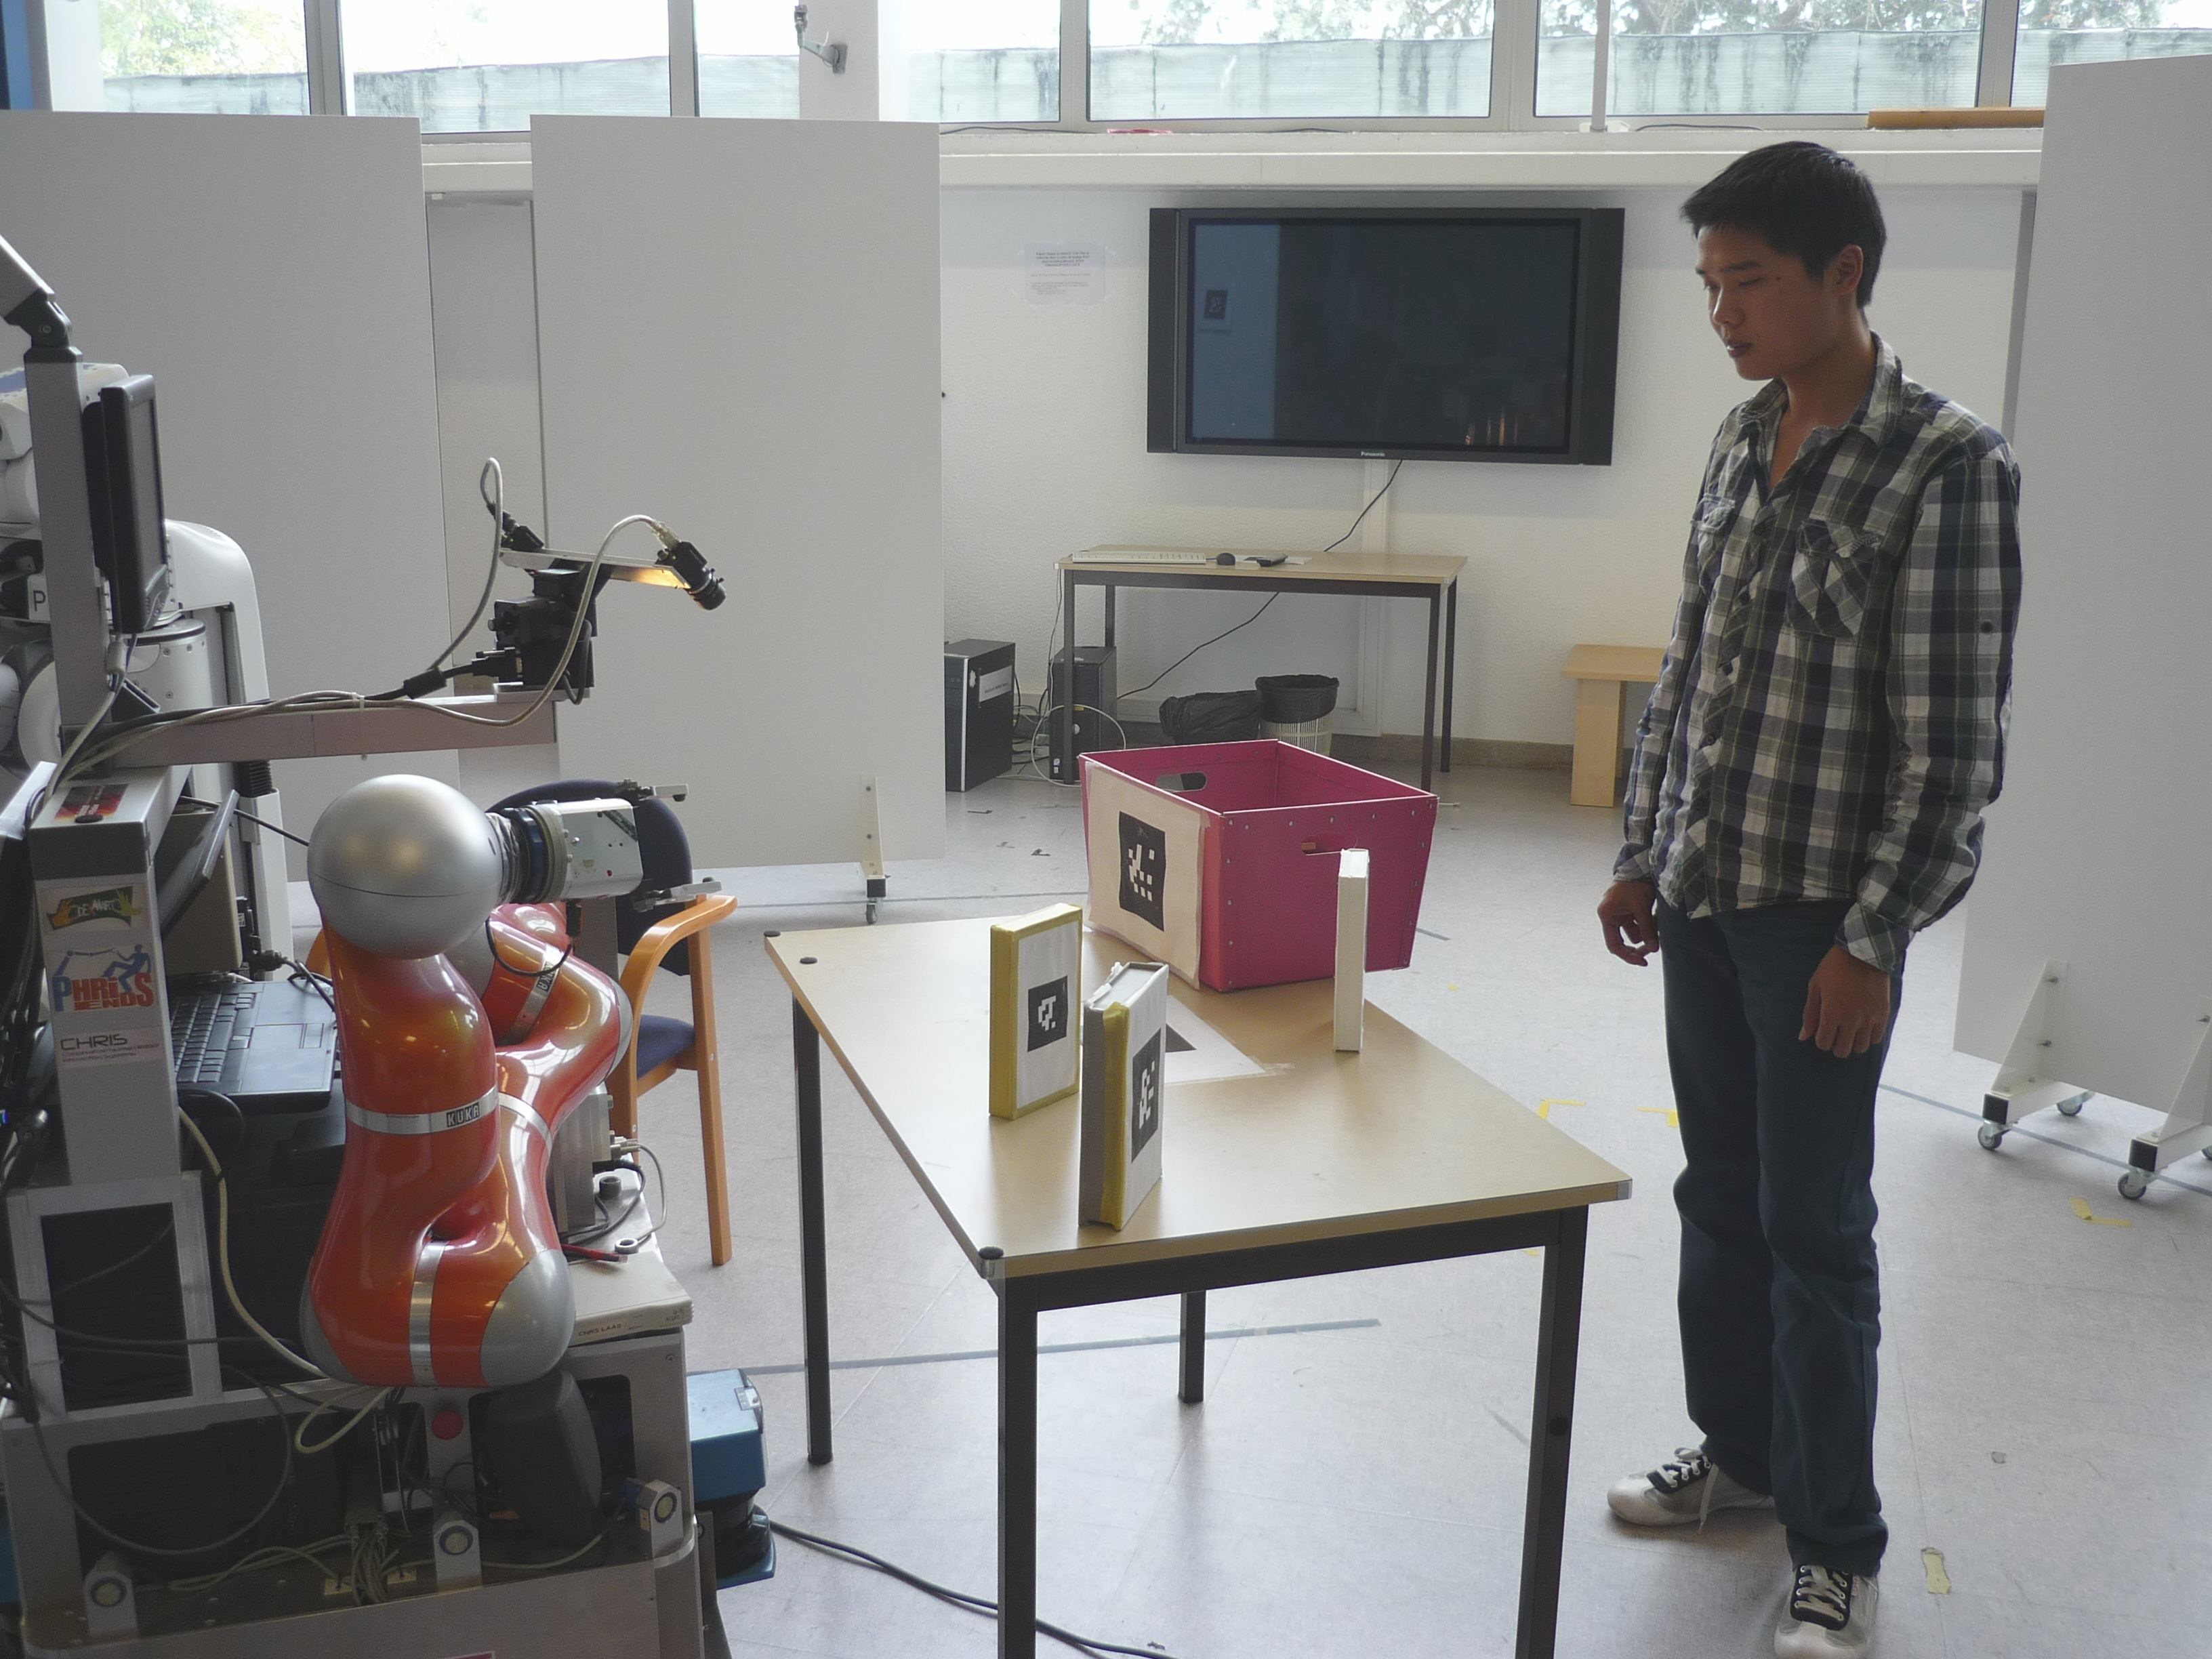
\includegraphics[width=0.5\textwidth]{spark/etat.jpg}
       }%
       \subfigure{%
          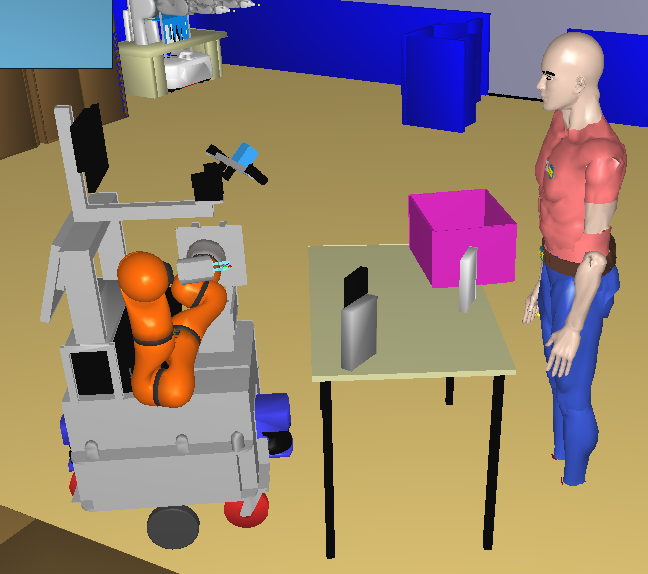
\includegraphics[width=0.43\textwidth]{spark/etat_spark.png}
       }\\ %  ------- End of the first row ----------------------%
%
   \end{center}

   \caption{The robot represents at runtime its environment in a 3D model
   resulting of the sensors' inputs fusion (Kinect, motion capture, 2D barcodes
   tracking).}

   \label{fig|spark}

\end{figure}

Figure~\ref{fig|spark} shows a screenshot of the SPARK environment side-by-side
with the real environment: as mentioned in the introduction, objects are
identified and localized through 2D barcodes. The human pose is tracked with
a Microsoft Kinect device (assisted by motion capture to accurately track the
head motion, which is required to compute what the human is looking at).

This geometric model is continuously updated at runtime by the robot.

\paragraph{Symbolic locations}

Human commonly refer to the positions of objects with symbolic descriptors
(like \emph{on}, \emph{next to}...) instead of precise, numeric position. These
type of descriptors have been studied in the context of language grounding
(\cite{O'Keefe1999,Matuszek2010,Regier2001,Kelleher2006,Blisard2005}). In this
work we focus agent-independent symbolic locations and agent-dependent,
relative locations.

\paragraph{Agent-independent locations}

We can refer to object locations with respect to other objects in the
environment, such as \emph{above, next to, in}, etc. In this work we compute
three main relations based on the bounding box and center of mass of the
objects (fig.~\ref{fig|sprelations}): 

\begin{itemize}
	\item \concept{isOn}: computes if an object $O_1$ is on another object $O_2$ by
	evaluating the center of mass of $O_1$ according to the bounding box of $O_2$.

	\item \concept{isIn}: evaluates if an object $O_1$ is inside another object
	$O_2$ based on their bounding boxes $BB_{O_1}$ and $BB_{O_2}$.

	\item \concept{isNextTo}: indicates whether an object $O_1$ is next to another
	object $O_2$. We cannot use a simple distance threshold to determine if two
	objects are next to each other since the relation is highly dependent on the
	dimensions of the objects. For instance, the maximum distance between large
	objects (\eg two houses) to consider them as being next to each other is much
	larger than the maximum distance we would consider for two small objects (\eg
	two bottles). Thus, the relation between the dimensions and the distances of
	the objects are taken into account.  

\begin{figure} 
	\centering
	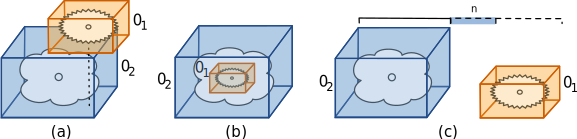
\includegraphics[width=0.95\columnwidth]{spark/spatial_relation.pdf}
	\caption{Spatial relations between two objects: (a) \concept{isOn} relation, 
	(b) \concept{isIn} relation, and (c) \concept{isNextTo} relation.} 
	\label{fig|sprelations} 
\end{figure}

\end{itemize} 

To ensure the different agent models are up-to-date, all these properties are
always computed on-line, each time the current state of the world changes.

Table~\ref{facts|sprelations} lists all the symbolic relationships that are
currently computed by the system.

\begin{table}[h]
    \centering
    \begin{tabular}{p{1.5cm}p{5cm}p{2cm}p{2.7cm}}
	\rowcolor{white}
    \textbf{Subject} & \textbf{Predicate} & \textbf{Object} & \emph{Notes} \\ 
    \hline
	 \concept{Location} & \concept{isAt} $\equiv$ \concept{cyc:objectFoundInLocation}  &  \concept{Location} & \\ 
	 &  $\rightarrow$ \concept{isOn} $\equiv$ \concept{cyc:above\_Touching}  &  & \\ 
	 &  $\rightarrow$ \concept{isIn}  &  & \\ 
	 &  $\rightarrow$ \concept{isNextTo}  & &  \\ 
	 \concept{Location}  & \concept{isAbove} $\equiv$ \concept{cyc:above-Generally}  &  \concept{Location}  &  inverse of \concept{isBelow} \par \concept{isOn} $\Rightarrow$ \concept{isAbove}\\ 
	 \concept{Location}  & \concept{isBelow}  & \concept{Location}  &  inverse of \concept{isAbove}
	\end{tabular}

	\caption{List of statements describing spatial relationships between
	objects. ``$\rightarrow$'' indicates sub-properties. When existing, the
	equivalent predicate in the {\sc OpenCyc} standard (prefix \concept{cyc:})
	has been added.}

\label{facts|sprelations}
\end{table}

SPARK also compute symbolic facts related to agent independent world dynamics.
The predicate \concept{isMoving} states, for each tracked entity, whether it is
currently moving or not.


\paragraph{Agent-dependent placements}

While in previous section we listed several \emph{absolute} location predicate,
many topological relations are directly dependent from the observation point.

The predicate \concept{hasRelativePosition} represents spatial locations
between agents and objects that are agent dependent.  For example we say ``it
is on my right, on your left, ...'' We compute these spatial locations by
dividing the space around the referent (an agent) into $n$ regions based on
arbitrary angle values relative to the referent orientation.  For example, for
$n = 4$ we would have the space divided into \emph{front, left, right} and
\emph{back}. Additionally, two proximity values, \emph{near} and \emph{far},
may also be considered. The number of regions and proximity values can be
chosen depending on the context where the interaction takes place.


To build an agent-dependent model of the world, \emph{Perspective
Taking}~\cite{Flavell1992,Tversky1999} is employed by the reasoner to provide
the robot with the ability to put itself at the human's place (by moving a
camera in the geometric model) and to reason about the world from different
perspectives.


Through perspective taking, SPARK computes for each agent a symbolic
description of the relative positioning of objects in the environment (table
\ref{facts|relative}).

\begin{table}[h]
	\centering
	    \begin{tabular}{p{1.5cm}p{6cm}p{1.5cm}l}
		\rowcolor{white}
		\textbf{Subject} & \textbf{Predicate} & \textbf{Object} & \emph{Notes} \\
		\hline
	 \concept{Location}  & \concept{hasRelativePosition}  & \concept{Location} & \\ 
	 & 	$\rightarrow$ \concept{behind} $\equiv$ \concept{cyc:behind-Generally}  &  & inverse of \concept{inFrontOf}  \\ 
	 &  $\rightarrow$ \concept{inFrontOf} $\equiv$ \concept{cyc:inFrontOf-Generally}  & 	 & 	 inverse of \concept{behind}  \\ 
	 &  $\rightarrow$ \concept{leftOf}  &  &  inverse of \concept{rightOf} \\ 
	 &  $\rightarrow$ \concept{rightOf}  & 	 & 	 inverse of \concept{leftOf}  \\ 
	 \concept{Object}  & \concept{cyc:farFrom}  &  \concept{Agent} & \\ 
	 \concept{Object}  & \concept{cyc:near}  &  \concept{Agent} & 
	\end{tabular}
	\caption{List of statements describing relative spatial relationships between objects and agents.}
	\label{facts|relative}
\end{table}


\subsubsection{Building a Model of Agents}
\label{sect|grounding_agents}

Building a grounded symbolic model of the physical environment does not suffice
in general to fully ground the human-robot interaction.

We divide the process of building models for agents into two categories:
operations related to the assessment of the current situation (for instance,
\emph{What does the human do? What does he see?}), and operations related to
the estimation of potential actions (for instance, \emph{Which regions could
the human reach if I want to hand over an object?}). We call these
potentialities of action \emph{Mightabilities}.

\paragraph{Agent Capabilities}

There are a number of common properties for a robot and a human related to
their capabilities in a given situation: they can both reach, grasp, look at,
point at, etc.: we group them in the \emph{Agent} category, defined as entities
that can act in the environment and manipulate it.

In this work we focus on the following capabilities from each agent's
perspective:

\begin{itemize}

\item \emph{Sees}: An important ability to know about an agent is to predict
\emph{What can it see?}, \ie what is within its field of view (FOV). A robot being
able to compute this information can then act accordingly. An example would be
a clarification scenario where the human is searching for an object and the
robot is able to infer that he/she is looking for the one that is not visible
(otherwise the user would not be searching for it).  In
Figure~\ref{fig::sparkRepresentations}\emph{a} the field of view of a person is
illustrated with a grey cone (broader one). While he is able to see the two
small boxes on the table in front of him, the big box on his right is out of
his FOV, and therefore, he is not able to see it. 

\item \emph{Looks At}: this relation corresponds to what the agent is focused
on, \ie where its focus of attention is directed. This model is based on a
narrower field of view, the field of attention (FOA). 
Figure~\ref{fig::sparkRepresentations}\emph{a}
shows the field of attention of a person with a green cone (narrower one). In
this example only the grey box satisfies the \concept{looksAt} relation.

\item \emph{Points At}: verifies whether an object is pointed at by an agent.
This relation is particularly useful during interaction when one of the agents
is referring to an object saying ``this" or ``that" while pointing at it.
 
If a larger object occludes a smaller one while an agent is pointing at them, the
outcome of the evaluation will result only in one relation, \ie \stmt{agent\_01
pointsAt object\_01} since the small one is not visible to the agent.  On the
contrary, if the small object is in front of the big one, then both objects
will satisfy the relation, which may generate an ambiguity (which object the
agent refers to?) that should be solved through higher level reasoning (\eg
context analysis or clarification through verbal interaction).

\item \emph{Reachable}: it allows the robot to estimate the agent's capability
to reach an object, which is fundamental for task planning. For example, if the
user asks the robot to give him/her an object, the robot must compute a transfer
point where the user is able to get the object afterward. 
Figure~\ref{fig::sparkRepresentations}\emph{b} shows different reachability postures for each object
on the table. In the example, the bottle and the box are both reachable for the
human, but the teddy bear is too far. Instead, from the robot's perspective,
the teddy bear is reachable, while the bottle is not.

\end{itemize}

\begin{figure*}[!t]
	\begin{center}
	\subfigure[]{
		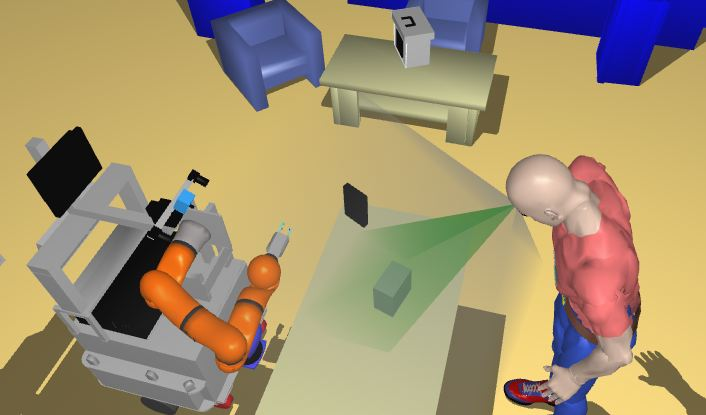
\includegraphics[width=0.4\linewidth]{spark/looks.jpg} 
	}
	\subfigure[]{
		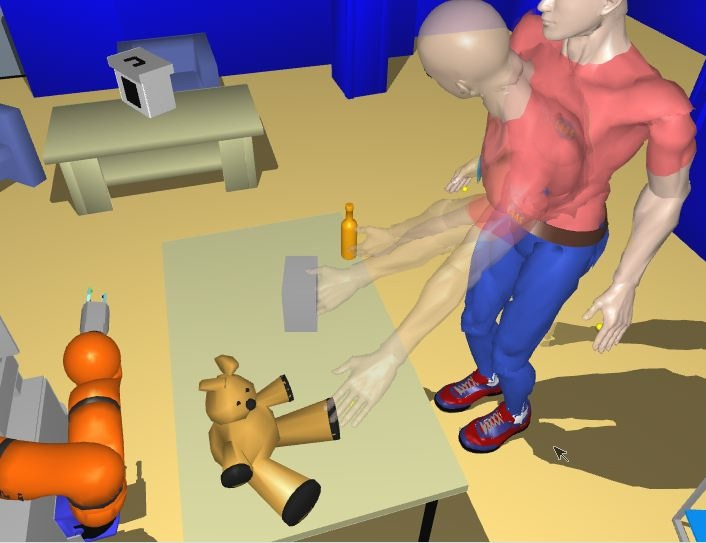
\includegraphics[width=0.35\linewidth]{spark/reach.jpg}
	} 
	\caption{(a) Field of view (FOV) and the field of attention (FOA) of the human. (b) Different reaching postures for the human.}
	\label{fig::sparkRepresentations}
	\end{center}
\end{figure*} 


While the first three relations (\concept{sees}, \concept{looksAt} and
\concept{pointsAt}) are computed through a model based approach, the latter one
is based on the Generalized Inverse Kinematics with pseudo inverse
method~\cite{Nakamura90,Baerlocher04} to find a posture for the
agent where its end-effector is at the center of the object within a given
tolerance.

Tables~\ref{facts|capabilites} summarizes the predicates produced by SPARK
during the agent capabilities analysis phase.

\begin{table}[h]
	\centering
		\begin{tabular}{p{2cm}p{4.5cm}p{2cm}p{3.5cm}}
		\rowcolor{white}
		\textbf{Subject} & \textbf{Predicate} & \textbf{Object} & \emph{Notes} \\
		\hline
		 \concept{Agent}  & \concept{looksAt}  & \concept{SpatialThing} \\
		 \concept{Agent}  & \concept{sees}  &  \concept{SpatialThing}  &    \\ 
		 \concept{SpatialThing}  & \concept{isInFieldOfView}  &  \concept{xsd:boolean}  & via inference: \par \stmt{myself sees *} $\Leftrightarrow$ \stmt{* isInFieldOfView true} \\ 
		 \concept{Agent}  & \concept{pointsAt} $\equiv$ \concept{cyc:pointingToward}  & \concept{SpatialThing} \\ 
		 \concept{Agent}  & \concept{focusesOn}  &  \concept{SpatialThing}  &  via inference: \par \concept{looksAt} $\wedge$ \concept{pointsAt} $\Rightarrow$ \concept{focusesOn} \\
		\concept{Agent} & \concept{seesWithHeadMovement} &  \concept{SpatialThing} \\
		\concept{Agent} & \concept{reaches} &  \concept{Object} \\ 

	\end{tabular}

	\caption{List of facts describing the attentional state and the abilities
	of an agent. \concept{looksAt} is interpreted as an object \emph{being in
	the field of attention} of an agent. An object is \concept{see}n if it is
	visible for the agent without moving the head (\ie, in \emph{field of
	view}).}

	\label{facts|capabilites}
\end{table}

Table~\ref{facts|agentstate} lists the other symbolic facts that are
produced and maintained by SPARK related to the general state of the agent.

\begin{table}[h]
	\centering
	\begin{tabular}{p{2cm}p{5cm}p{2cm}}
		\textbf{Subject} & \textbf{Predicate} & \textbf{Object} \\
		\hline
		\concept{Agent} & \concept{hasIn\{Left|Right\}Hand}  &  \concept{GraspableObject} \\ 
		\concept{Agent} & \concept{hasPosture}  &  \concept{Posture} \\
		\concept{Agent} & \concept{currentlyBodilyDoes}  &  \concept{Action}
	\end{tabular}

	\caption{List of statements describing the state of an agent in general.
	\concept{Posture} can be either \concept{standing} or \concept{sitting}.
	The \concept{currentlyBodilyDoes} predicate states the current action of
	the agent, be it intentional or not.}

	\label{facts|agentstate}
\end{table}

%%%%%%%%%%%%%%%%%

\subsection{Integration with symbolic task planning and executive layers}

\subsubsection{Symbolic Task Planning}
\fxnote{HATP}

\subsubsection{Execution Control}
\fxnote{CRAM, SHARY, pyrobots, RAD...}

\subsection{Integration with natural language processors}

%%%%%%%%%%%%%%%%%

\subsection{Towards an Event-Driven, Knowledge-Oriented Architecture}

In this section, we have presented how knowledge streams are organized between
several components: {\it(1)} {\sc ORO}, the ontology-based knowledge server
that stores and maintains classified RDF statements produced by other modules
in agent-specific models and allows information to be retrieved either through
queries or via an event system; {\it(2)} {\sc SPARK}, the grounded,
human-aware, 3D model of the environment that performs all the spatial
reasoning within this architecture, including reasoning involving motion
planing (to compute reachability of objects) and perspective taking, {\it(3)}
{\sc CRAM}, {\sc SHARY}, {\sc pyRobots}, {\sc RAD}, {\sc HATP} as differents
examples of execution controllers and symbolic task planners that take
advantage of semantic abstractions provided by knowledge base and {\it(4)} {\sc
Dialogs}, a natural language processor that performs simple grammatical parsing
of English language, grounds the semantic content of the utterance (if
necessary, also interacts with the user to disambiguate), and eventually
generates a RDF representation of the sentence.

Altogether, these components compose an architecture that we call
\emph{knowledge-oriented}:

\begin{itemize} \item{Knowledge is explicitly stored in one central and
consistent repository of facts, accessible by all modules.} \item{Knowledge is
represented in a strict formalism (OWL statements) and with a clearly defined
vocabulary (stated in the {\tt commonsense.oro.owl} ontology).} \item{The first
two points enable both a loosely-coupled architecture where modules can very
easily be removed or replaced by other ones as long as they share the same
semantics (modules are defined by the knowledge they produce),} \item{and a
\emph{symbolic} reactive, event-driven approach to supervision. By managing
events at the same level as the reasoner, we take full advantage of the
inference abilities of ORO to trigger events whose \texttt{true} conditions can
be inferred.} \item{Finally, this architecture allows for the combination of
very different knowledge modalities in a single homogeneous environment,
bringing mutual benefits to components. For instance, the dialogue processing
module can perfectly run without any geometric perception, but its
disambiguation routines can transparently benefit from it when available (since
richer symbolic descriptions of objects are then available).} \end{itemize}

This architecture moves away from standard layered approaches. Interactions
between components are mostly bidirectional and, from the software components
point of view, we do not introduce layers of abstraction (we do, however, have
access to the lower level modules of the robot to execute actions, but all
cognition-related modules reside at the same level). This is especially visible
for the dialogue input processing. This component does not simply act as an
alternative perceptual input to the symbolic database, but also actively
queries previously acquired knowledge to disambiguate and validate the newly
created symbolic knowledge, as we will present in details in the following
chapter.

Regarding the anchoring question, this architecture is bidirectional. The
components we described provide a \textit{bottom-up} grounding process: SPARK
and \textsc{Dialogs} constantly build and push new symbolic contents about the
world to ORO where it becomes accessible to decisional layers. In parallel, ORO
relies on reasoning in a \textit{top-down} way to produce new facts that may
trigger in return physical behaviours. 

We believe that this \emph{knowledge-oriented} approach has a strong potential
not only to enable rich human-robot interaction, but also as a broader approach
to information alignment and fusion in complex robotic systems.  The
versatility of this paradigm could be illustrated by a simple imaginary
scenario with a blind robot and a deaf robot. The blind robot does not see (no
cameras or alike), but someone can verbally describe a scene to it. On the
other hand, the deaf robot has a good vision system, but cannot process verbal
input.  Without any changes to the software architecture that we described,
supervision modules of both robots would be able to perform equally well (to
actually implement this imaginary situation, the blind robot would of course
need \textit{a priori} 3D models of objects talked about to enable planning or
pick and place actions, and the deaf robot would require at least some gesture
interpretation to understand orders).

This architecture may also contribute to bridge the gap between robotics and
psychology: it provides clear entry points to implement some classical
psychology tests to robots. We presented experiments focused on issues related
to perspective taking. By explicitly enabling independent modeling of the
beliefs of each agent, our architecture is especially well suited to set up
cognitive and psychological experiments (such as the \emph{False-Belief}
experiment), which we plan to further explore.
